\chapter{Real Estate: Control Before Ownership}

This chapter draws from the School of Hard Knocks interview with Matt Teifke, curated by LazyingArt LLC through Video2Book. The transcript is not a blackboard lecture, and no validated mathematical screenshots remain. The useful structure is therefore commercial rather than formal physics: wage income versus commission income, agent splits, licensing thresholds, partnership roles, contract control, tax drag, and risk. We will keep the spoken order of the interview and treat each number as testimony from the source, not as legal, financial, or investment advice.

\section{The Check That Reframed the Game}

The interview opens before it introduces itself. We first hear the payoff image: a local broker receives a \(\$200{,}000\) check while Matt Teifke is sitting there, turns it around, and tells him that he will get there one day. Then the scene cuts to the other end of the ladder: Matt is working at Papa John's, delivering pizza and mopping the floor, when the first real estate call comes in.

That ordering matters. Before we know the school, the licenses, the brokerage, or the later company, we know the discontinuity in income scale. The first mechanism is not yet sophisticated ownership. It is commission income attached to a closed transaction.

Let \(W\) denote a rough wage-job paycheck and \(C_1\) the first real estate commission Matt reports. The transcript gives

\begin{equation}
W_{\text{pizza check}} \approx \$600,
\qquad
C_1 \approx \$6{,}000 \text{ to } \$7{,}000 .
\end{equation}

As a scale comparison, not an exact life-income calculation,

\begin{equation}
\frac{\$6{,}000}{\$600}=10,
\qquad
\frac{\$7{,}000}{\$600}\approx 11.7 .
\end{equation}

So the first lesson is not simply that real estate ``pays more.'' It is that a different compensation rule is being encountered. A pizza job pays for time and shifts. A commission pays when a transaction closes. The narrative force of dropping the mop is that the call belongs to a different game.

\section{Learning Real Estate Until Ownership Became the Question}

After the preview, the host formally names Matt as the owner of Teifke Real Estate and frames the goal: to build an entrepreneurial real estate brokerage. Matt then walks backward through the preparation. He was born in Cleveland, moved to Austin as a child, grew up with a single mother, and says his mother showed him what was possible in real estate.

The path is cumulative. He got licensed at 17, went to Texas A\&M Corpus Christi, worked at a mom-and-pop brokerage, earned rookie of the year while a full-time student, worked for a commercial brokerage in Round Rock, then went to Texas A\&M for a master's degree in real estate. He emphasizes that the master's was financially based. He also worked at an apartment property and got an appraisal license.

The repeated question beneath the biography is: how do we move from knowing about real estate to owning or controlling real estate? Matt says this directly. He wanted to learn as much as possible, then figure out how to own real estate.

The first company he started with his wife was third-party property management. Its scale is given as

\begin{equation}
D_{\text{managed}}=700 \text{ doors}.
\end{equation}

That company was later sold. The next step was not simply another job. He teamed up with Alex Kaufman, a childhood friend, and built the entrepreneurial brokerage that frames the interview.

\subsection{Question \& Answer}

\paragraph{Question.}
Is college necessary for success in this path, or did it transfer into the skills of owning a brokerage and finding deals?

\paragraph{Answer.}
Matt's answer is deliberately conditional: necessary, no; useful, yes, if one uses it. He describes teaching a college class and telling students that ten people in a room who are all interested in business could help one another for life. The missed opportunity is not that students lack credentials. It is that many simply show up to class and leave.

The mechanism is therefore not a diploma by itself. It is a network and a repeated opportunity environment. In compact form, the claim is

\begin{equation}
\text{College value} \neq \text{degree alone};
\qquad
\text{college value} \approx \text{skills}+\text{network}+\text{initiative}.
\end{equation}

This should not be overstated as a universal theorem. It is Matt's practical interpretation of his path: college was not strictly required, but it could become valuable if converted into relationships, financial understanding, and deal flow.

\section{The First Deal and the Reversal of the Interview}

The host then takes Matt back to the first real money-making moment in real estate. Matt explains that as a young prospective agent he misunderstood the labor market. He set up interviews with brokerages, showed up in a suit and tie, and hoped they would give him a job. Later he realized the structure was almost inverted: brokerages often want new agents.

This is the second important commercial reversal. The broker is not only evaluating the agent; the brokerage also benefits from agents who bring in transactions. That is why the \(\$200{,}000\) check is such a powerful image. It demonstrates the ceiling of the transaction world before Matt has even entered it.

The first closing then makes the lesson concrete. Matt says he was still working at Papa John's because he needed money. He got the call while mopping, took it, closed, and made about \(\$6{,}000\) or \(\$7{,}000\). He compares that with ordinary checks of about \(\$600\), and even with larger earlier full-time checks of perhaps \(\$1{,}500\) or \(\$2{,}000\).

The important distinction is between income as wage and income as event. If \(C\) is commission from a closed deal, then a brokerage split later decides who keeps what fraction of \(C\). But at this first stage the breakthrough is simply that \(C\) exists.

\section{From Agent to Broker}

The next question is natural: if the start is as an agent, how does one move toward owning a brokerage? Matt answers by distinguishing the licensed agent from the broker. As he describes it, every licensed agent must have a broker. The broker is the person or entity under whose responsibility the agent operates.

\subsection{Question \& Answer}

\paragraph{Question.}
How does the transition from agent to broker work?

\paragraph{Answer.}
Matt describes the rule as he experienced it. When he started, it was two years plus a certain amount of sales to obtain a broker's license. Just before he reached the two-year mark, the requirement changed to four years. He then describes a transaction point system, saying he believes it required about 900 points, along with real estate classes and qualifying credit hours. His college degree and master's degree satisfied those credit hours. After the required transactions and test, he became licensed.

We should state this carefully. These are not current legal instructions; they are the path as Matt recounts it. In notation,

\begin{equation}
T_{\text{experience}}=4\text{ years},
\qquad
P_{\text{points}}\approx 900 .
\end{equation}

The transition is not merely a status change. Once licensed as the broker, one becomes responsible: on the hook, training agents, supporting agents, and absorbing the risks that arrive when transactions become complicated.

\begin{table}
\centering
\begin{tabular}{|p{0.32\linewidth}|p{0.56\linewidth}|}
\hline
Stage & Function in Matt's description \\
\hline
Licensed agent & Must operate under a broker; earns through closed transactions. \\
\hline
Broker candidate & Accumulates experience time, transactions, points, classes, credit hours, and passes the test. \\
\hline
Broker & Carries responsibility, trains and supports agents, and participates in the brokerage split. \\
\hline
\end{tabular}
\caption{Transcript-grounded reconstruction of the agent-to-broker ladder.}
\end{table}

The economics of the brokerage appear immediately after the licensing discussion. Matt says his current brokerage uses a 90-10 split: the agent keeps 90 percent, the brokerage takes 10 percent. His first brokerage, by contrast, was 50-50. If \(C\) is a gross commission from a closed deal, the two structures are

\begin{align}
\text{Current split:}\qquad
C_{\text{agent}}&=0.90C,
&
C_{\text{brokerage}}&=0.10C,\\
\text{First brokerage:}\qquad
C_{\text{agent}}&=0.50C,
&
C_{\text{brokerage}}&=0.50C.
\end{align}

This is a simple equation, but it carries a business philosophy. A brokerage can extract heavily from each transaction, or it can make itself attractive to entrepreneurial agents by giving them a larger share while trying to scale through volume, culture, training, and support.

\section{Being on the Hook}

The host then asks about the hardest part of owning a brokerage. The answer moves from formal requirements to lived responsibility. Matt says the hard part is leading the team while carrying one's own challenges. Deals fall apart. Lawsuits appear. Complaints arrive. The broker still has to show up and lead.

This section is the moral counterpart of the 90-10 split. The brokerage takes a percentage, but the percentage is not free money. It corresponds to responsibility, training, support, supervision, and liability. We can express the role schematically:

\begin{equation}
\text{Brokerage claim on } C
\quad \longleftrightarrow \quad
\text{support}+\text{training}+\text{risk bearing}+\text{leadership}.
\end{equation}

This is not an accounting identity. It is the mechanism Matt is describing. The broker owns a structure, and the structure includes pressure. The chapter should preserve this transition: first the credential, then the split, then the burden.

\section{Partnership as Operating Design}

The next major beat is partnership. The host notes that Matt has a partner, Alex, and asks what it is like to work in that partnership and what qualities matter in a business partner. Matt starts with a stark claim: one in twenty partnerships work out, if that.

Then he gives the story rather than a rule. Alex was a childhood connection, someone Matt had known since he was young. Matt describes Alex's heroin addiction, jail, recovery, and the caution Matt felt when they first started working together. The trust was not granted at once. It was tested.

The tests were behavioral. Matt would give Alex 10 doors to knock, and Alex would knock 100. He would ask him to call people, and Alex would call ten times the number. Over two or three years, they ended up owning four or five properties together.

\begin{align}
10\text{ doors assigned} &\longrightarrow 100\text{ doors knocked},\\
1\text{ unit of calling requested} &\longrightarrow 10\text{ units of calling performed},\\
2\text{ to }3\text{ years} &\longrightarrow 4\text{ to }5\text{ jointly owned properties}.
\end{align}

The story then becomes an operating model. Alex is described as the operations person: counting the money, making sure the firm is profitable, hiring, and firing when needed. Matt describes his own best role as networking, building relationships, talking to people, and generating new ideas. He says they operate through Traction language: Alex as implementer, Matt as visionary.

\begin{figure}
\centering
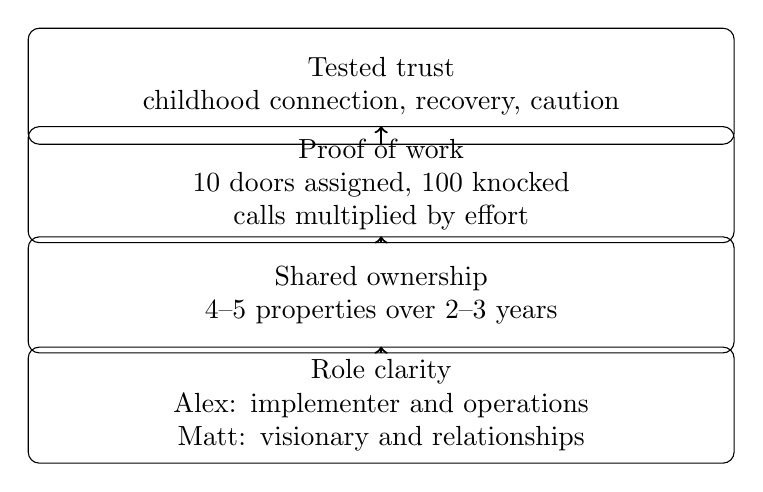
\begin{tikzpicture}[
  box/.style={draw, rounded corners, align=center, text width=0.72\linewidth, minimum height=0.58in},
  arrow/.style={->, thick}
]
\node[box] (trust) at (0,0) {Tested trust\\childhood connection, recovery, caution};
\node[box] (proof) at (0,-1.25) {Proof of work\\10 doors assigned, 100 knocked\\calls multiplied by effort};
\node[box] (assets) at (0,-2.65) {Shared ownership\\4--5 properties over 2--3 years};
\node[box] (roles) at (0,-4.05) {Role clarity\\Alex: implementer and operations\\Matt: visionary and relationships};
\draw[arrow] (trust) -- (proof);
\draw[arrow] (proof) -- (assets);
\draw[arrow] (assets) -- (roles);
\end{tikzpicture}
\caption{Transcript-grounded reconstruction of how the partnership becomes an operating design.}
\end{figure}

This is one of the lecture's strongest practical mechanisms. The right partner is not defined by charisma. The partner becomes credible through repeated evidence under small tests, then the partnership becomes scalable when roles stop overlapping.

\section{The Wholesale Deal}

The host then asks about best and worst financial decisions and, inside that, the biggest deal. Matt answers the biggest-deal question first: a \(\$700{,}000\) to \(\$780{,}000\) wholesale fee, made between three partners. The host pauses to ask for an explanation of wholesaling, and that pause should remain in the chapter because the answer is the clearest transaction model in the interview.

\subsection{Question \& Answer}

\paragraph{Question.}
What is wholesaling in this example?

\paragraph{Answer.}
Matt's account is specific. They put a property under contract. The seller did not want brokers, so they took off the broker hat and approached the deal as investors. The contract price was about \(\$2{,}000{,}000\). They had a 3 percent commission going to themselves. They put up earnest money and option money of about \(\$20{,}000\). In Matt's language, they then controlled the piece of paper, and that control functioned as ownership of the opportunity.

Let

\begin{equation}
P_{\text{contract}}=\$2{,}000{,}000,
\qquad
E+O\approx \$20{,}000,
\qquad
A=9.5\text{ acres}.
\end{equation}

They called builders, developers, and anyone who might be interested. The property was nine and a half acres in Round Rock, and Matt says they also wanted to own it themselves because it was a commercial property. They then received an offer at about \(\$2{,}700{,}000\):

\begin{equation}
P_{\text{offer}}=\$2{,}700{,}000.
\end{equation}

A cautious reader-aid reconstruction of the gross spread is

\begin{align}
\Delta P
  &=P_{\text{offer}}-P_{\text{contract}}\\
  &=\$2{,}700{,}000-\$2{,}000{,}000\\
  &=\$700{,}000.
\end{align}

Matt reports the wholesale fee as \(\$700{,}000\) to \(\$780{,}000\), and later says they made the 700K. The range should be preserved rather than forced into one exact number:

\begin{equation}
F_{\text{wholesale}}\approx \$700{,}000\text{ to }\$780{,}000.
\end{equation}

He also says they made the 3 percent commission. If we compute that on the stated \(\$2{,}000{,}000\) contract price, the reconstruction is

\begin{equation}
C_{\text{commission}}
=
0.03 \times \$2{,}000{,}000
=
\$60{,}000.
\end{equation}

That commission-base assumption should remain cautious. The transcript gives the 3 percent figure, but does not spell out every closing statement line.

\begin{figure}
\centering
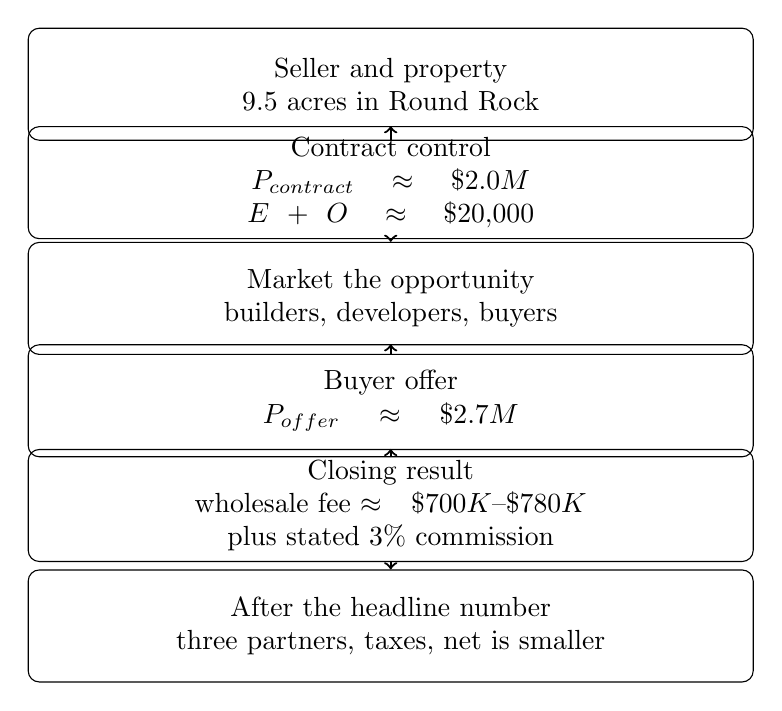
\begin{tikzpicture}[
  box/.style={draw, rounded corners, align=center, text width=0.74\linewidth, minimum height=0.56in},
  arrow/.style={->, thick}
]
\node[box] (seller) at (0,0) {Seller and property\\9.5 acres in Round Rock};
\node[box] (contract) at (0,-1.25) {Contract control\\\(P_{\text{contract}}\approx \$2.0\text{M}\)\\\(E+O\approx \$20{,}000\)};
\node[box] (market) at (0,-2.72) {Market the opportunity\\builders, developers, buyers};
\node[box] (offer) at (0,-4.02) {Buyer offer\\\(P_{\text{offer}}\approx \$2.7\text{M}\)};
\node[box] (close) at (0,-5.35) {Closing result\\wholesale fee \(\approx \$700\text{K}\)--\(\$780\text{K}\)\\plus stated 3\% commission};
\node[box] (after) at (0,-6.88) {After the headline number\\three partners, taxes, net is smaller};
\draw[arrow] (seller) -- (contract);
\draw[arrow] (contract) -- (market);
\draw[arrow] (market) -- (offer);
\draw[arrow] (offer) -- (close);
\draw[arrow] (close) -- (after);
\end{tikzpicture}
\caption{Transcript-grounded reconstruction of the wholesale-control sequence.}
\end{figure}

The lesson is not that every wholesale deal produces this result. Matt himself says it did not feel real until closing and that the tax bill made it less than it seemed. The mechanism is narrower and more durable: control can precede ownership. The valuable asset in the middle of the deal was not yet the land itself; it was the contract position and the ability to transfer it.

If the fee is split evenly among three partners, a rough pre-tax share is

\begin{equation}
\frac{F_{\text{wholesale}}}{3}
\approx
\$233{,}333 \text{ to } \$260{,}000,
\end{equation}

before taxes and before resolving the exact treatment of the commission. This is a reconstruction for scale only. The transcript does not give the partners' final net proceeds.

\section{Risk, Regret, and Motivation}

After the wholesale explanation, the host circles back to best and worst financial decisions. Matt says he has perhaps 130 properties, but names the worst decision as cannabis stock. He says he is down multiple millions, and describes daily movements of \(\$60{,}000\) to \(\$100{,}000\).

\begin{equation}
L_{\text{total}}=\text{multiple millions},
\qquad
\Delta L_{\text{daily}}\approx \$60{,}000\text{ to }\$100{,}000.
\end{equation}

He names Acreage and says he still believes in the company and the industry. He states that the company did \(\$67{,}000{,}000\) in revenue last quarter while being valued at \(\$40{,}000{,}000\). We can record the comparison as testimony:

\begin{equation}
R_{\text{quarter}}\approx \$67{,}000{,}000,
\qquad
V_{\text{company}}\approx \$40{,}000{,}000.
\end{equation}

A purely arithmetic ratio would be

\begin{equation}
\frac{R_{\text{quarter}}}{V_{\text{company}}}
\approx
1.675.
\end{equation}

But this should not be turned into investment advice. It is Matt's way of explaining why he still believes the position might be early rather than wrong, while also admitting the mark-to-market pain.

His best financial decision is not a stock, property, or trade. It is partnering with Alex. That answer ties the risk section back to the earlier partnership section: the most important compounding asset in this account is not only a deal skill, but a trusted operating relationship aimed at a clear goal.

The interview then asks for a wild real estate story. Matt tells one about his pregnant wife being chased at a managed property, and another about negotiating a deal with someone at an RV park over a beer. The point is not merely color. Real estate, in this telling, is full of irregular human situations. The operator has to treat strange days as part of the terrain.

The final question asks about the next ten years and motivation. Matt's answer returns to clarity. He says he is driven, influenced by his mother, and blessed to have a clear vision. He does not say that he is always on fire. He says the goal is clear, and that agents tell them the brokerage changed their lives. That daily feedback keeps the work going.

\section{Summary}

The lecture moves through a clean sequence of commercial mechanisms. First, Matt encounters commission income as a scale change from wage work. Then he accumulates real estate fluency through licenses, college, brokerage work, appraisal, property management, and a 700-door company. The college discussion becomes a lesson about turning environments into networks rather than merely collecting credentials.

The middle of the interview explains the move from agent to broker: experience, transactions, points, classes, credit hours, testing, and then responsibility. The 90-10 split is meaningful only when paired with the burden of being on the hook. Partnership then becomes an operating design, not a slogan: small tests, overdelivery, shared ownership, and divided roles.

The biggest deal gives the sharpest quantitative example. A \(\$2{,}000{,}000\) contract position, about \(\$20{,}000\) of earnest and option money, outreach to buyers, and a \(\$2{,}700{,}000\) offer created a reported \(\$700{,}000\) to \(\$780{,}000\) wholesale fee, before partner splits and taxes. The final lesson is that wealth in this interview is not presented as clean abstraction. It is built from control, relationships, repeated action, risk, taxes, and a goal clear enough to keep returning to.